\chapter{Revisão Bibliográfica}\label{cap:fundament}



Esse capítulo tem como objetivo apresentar conceitos que facilitarão o entendimento do conteúdo do Capítulo \ref{cap:solucao}, detalhando técnicas e conceitos utilizados na execução do trabalho através de exemplos e imagens. Serão apresentados conceitos relacionados ao processamento de imagens estáticas, seguidos de uma discussão breve sobre técnicas aplicadas em vídeos e conceitos de redes neurais artificiais e classificação de padrões. O capítulo finaliza com uma rápida apresentação de trabalhos correlatos.
 %O conteúdo deste capítulo continua no Cápitulo \ref{cap:redes} que apresenta conceitos de redes neurais e classificação de padrões. 


\section{Fundamentação Teórica}

\subsection{Processamento de Imagens}\label{sec:processamento}

\subsubsection{Imagens em nível de cinza}

Para que um computador seja capaz de operar sobre uma imagem, é preciso que seja utilizado um modelo de representação que traduza o que os nossos sentidos conseguem perceber em informações que podem ser interpretadas por uma máquina que não é dotada de visão. A forma mais simples de se representar uma imagem são as imagens em nível de cinza. Podemos definir imagens como uma função \textit{f{(x,y)}} onde x e y são coordenadas espaciais e o valor de  \textit{f{(x,y)}} é a luminosidade, ou nível de cinza, da imagem naquele ponto. Quando esses valores são todos discretos, chamamos essa imagem de uma imagem digital~\cite{gonzalez2009digital}. Cada elemento individual dessa imagem, cada valor em cada coordenada, pode ser chamado de um \textit{picture element} ou mais comumente \textit{pixel}. Em imagens digitais em nível de cinza, cada \textit{pixel} possui 1 \textit{byte} de informação, ou seja, pode assumir valores entre 0 e 255, onde o valor 0 representa o preto e 255 representa o branco. 

Uma imagem então, pode ser interpretada por um programa de computador como uma matriz $M\times N$ de elementos de 1 \textit{byte}, onde $M$ é a largura da imagem e $N$ é a sua altura. Cada elemento $p_{i,j}$ da matriz possui a informação de luminosidade do pixel correspondente e o computador é capaz de exibir e interpretar esses valores apropriadamente. A Figura \ref{fig:NivelCinza} exemplifica esse processo.

\begin{figure}
 \centering
\begin{subfigure}{.5\textwidth}
  \centering
  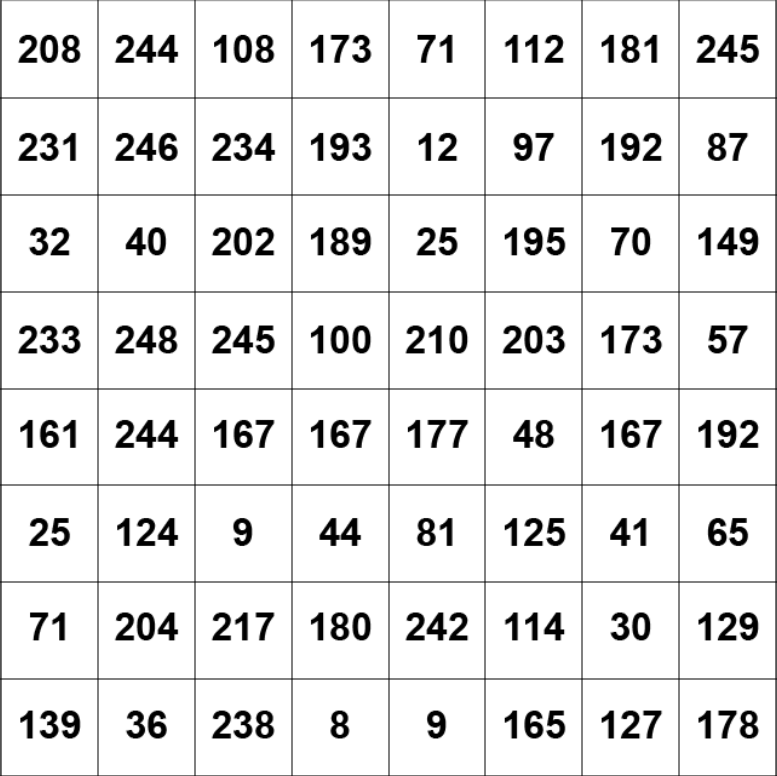
\includegraphics[width=.5\linewidth]{MatrizNivelCinza}
  \caption{}
  \label{exemplo:sfig1}
  \centering
\end{subfigure}%
\begin{subfigure}{.5\textwidth}
  \centering
  
\includegraphics[width=.5\linewidth]{ExemploNivelCinza}
  \caption{}
  \label{exemplo:sfig2}
  \centering
\end{subfigure}
\caption{(a) Uma matriz com níveis de cinza e (b) a imagem correspondente.}
\label{fig:NivelCinza}
\centering
\end{figure}


\subsubsection{Espaços de cores}

Para que um sistema de processamento de imagens possa interpretar e processar cores, é preciso criar modelos apropriados para representá-las. Chamamos os modelos de representação das cores em uma imagem um espaço de cor. Existem diversos espaços de cor, cada um importante para a realização de tarefas e necessidades diferentes~\cite{acharya2005image}. Para a compreensão deste trabalho, é necessário, porém, entender apenas dois: o espaço RGB e o espaço YCbCr.

\subsubsection{O espaço RGB}


RGB é um acrônimo para \textit{Red, Green, Blue}, vermelho, verde e azul em inglês. Essas cores são consideradas então cores primárias aditivas devido ao fato de pesquisas mostrarem que um grande gama de cores pode ser formado através de combinações aditivas das cores vermelho, verde e azul~\cite{IBGE2000introducao}. Nesse modelo, a cor de um \textit{pixel} de uma imagem é representada através de três coeficientes que definem a influência de cada cor primária na combinação. Uma imagem no modelo RGB é então representada por três matrizes de níveis de cinza de dimensões iguais, chamadas canais, onde cada valor representado na matriz, representa o valor do coeficiente da cor correspondente na imagem final. Isto é, a imagem pode ser representada por uma matriz $M\times N\times 3$ onde a cor final $C_{i,j}$ de cada \textit{pixel} da imagem é definida pela Equação \ref{eq:corRGB}. Se os coeficientes são representados por um \textit{byte}, é possível então representar aproximadamente $16,7$ milhões de cores com este modelo. A Figura \ref{fig:Espacos:sub:RGB} mostra os canais de uma imagem RGB separadamente.

Esse espaço de cor é o mais comumente usado para representar imagens que vemos no cotidiano, uma vez que é semelhante a visão humana e portanto é utilizado pelos dispositivos multimídia mais comuns.
	
	\begin{equation}
			C_{i,j} = p_{i,j,1} . R + p_{i,j,2} . G + p_{i,j,3} . B ,  (1\leq i\leq M, 1\leq j\leq N)
	\label{eq:corRGB}
	\end{equation}

\subsubsection{Espaço YCbCr}\label{sect:sub:ycbcr}

Assim como o espaço de cor RGB, o espaço YCbCr também representa uma imagem através de três matrizes, porém, seus canais contém informações diferentes do modelo RGB. Esse modelo é muito utilizado para o armazenamento de vídeos, uma vez que o modelo tira vantagem de alguns aspectos da visão humana para poder armazenar menos dados, sem perda significativa de informação visual. Por exemplo, humanos são mais sensíveis à detalhes e variações em níveis de cinza do que detalhes em imagens coloridas. Além disso, o olho humano é mais sensível ao verde do que qualquer outra cor~\cite{colorSpacesDigitalVideo}. Com esse conhecimento, o espaço YCbCr representa as cores de uma imagem através de sua luminosidade (Y) e os valores de crominância azul (Cb) e crominância vermelha (Cr). Cb e Cr são sinais de diferença de cor e são definidos pela subtração do valor de luminosidade do canal azul e vermelho da imagem, respectivamente. A luminosidade é definida pela Equação \ref{eq:Y}~\cite{LivroVideoDigital} que reflete a sensibilidade maior a cor verde da visão humana.

Na Figura \ref{fig:Espacos:sub:YCbCr} estão exemplificados os canais de uma imagem no espaço YCbCr.

\begin{equation}
	Y = 0,299.R + 0,587.G + 0,114.B
\label{eq:Y}
\end{equation}


\begin{figure}
 \centering
\begin{subfigure}{.5\textwidth}
  \centering
  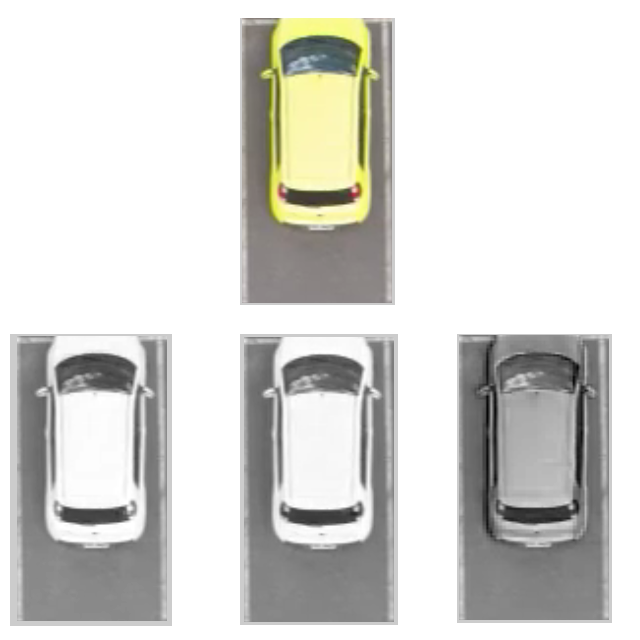
\includegraphics[width=.8\linewidth]{exemploRGBFinal}
	\caption{}
	\label{fig:Espacos:sub:RGB}
	\centering
\end{subfigure}\
\begin{subfigure}{.5\textwidth}
  \centering
  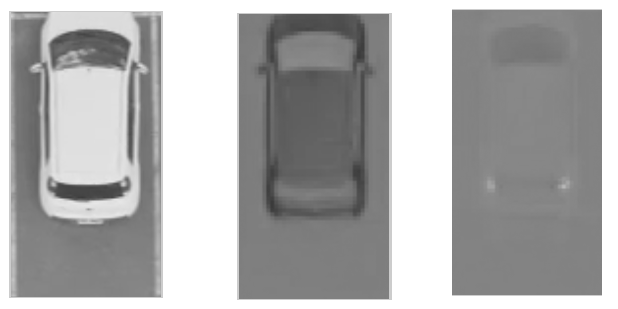
\includegraphics[width=.8\linewidth]{exemploYCbCrFinal}
	\caption{}
	\label{fig:Espacos:sub:YCbCr}
	\centering
\end{subfigure}
\caption{(a) Uma imagem e cada um de seus canais RGB ordenados da esquerda para a direita e (b) os canais YCbCr da imagem ordenados da esquerda para a direita.}
\label{fig:Espacos}
\centering
\end{figure}

\subsubsection{Descritores de textura}\label{sec:descritores}

Descritores de textura são algoritmos que procuram fazer o que o olho humano faz com facilidade: distinguir tipos diferentes de objetos apenas por algumas de suas características visuais~\cite{GLCM}. Estes algoritmos observam e analisam características pertinentes a imagem inteira e são capazes de identificar diferenças mais sutis entre imagens diferentes. Existem diversas técnicas de descrição de textura~\cite{ojala2002multiresolution} que são utilizadas com sucesso em aplicações de processamento de imagem. Para esse trabalho, a técnica escolhida foi a conhecida como GLCM (\textit{gray-level co-ocurrence matrix}) descrita na Seção \ref{sec:GLCM}, por ter execução rápida e ser invariante quanto à escala de cinza.

\subsubsection{GLCM}\label{sec:GLCM}

GLCM, ou matriz de co-ocorrência de nível de cinza, é uma técnica de descrição de textura que visa extrair medidas estatíticas da imagem sendo analisada. Para tanto, é criada uma matriz quadrada de tamanho $M\times M$ onde M é a quantidade de níveis de cinza possíveis na imagem em questão. Essa matriz armazena a probabilidade de dois \textit{pixels} se relacionarem através de uma certa relação espacial~\cite{GLCM}. 

Para esse trabalho, a relação observada é a da vizinhança entre dois \textit{pixels}, sempre analisando o valor a direita de um determinado \textit{pixel} da imagem. Os 255 valores de intensidade possíveis são divididos em 8 níveis. Cada elemento $P_{(a,b)}$ na GLCM $G$ conta a quantidade de vezes que um \textit{pixel} com valor de intensidade  $a$ apareceu à direita de um \textit{pixel} com valor $b$. A Figura \ref{fig:GLCM} exemplifica a criação da GLCM a partir de uma imagem com 8 níveis possíveis.

\begin{figure}
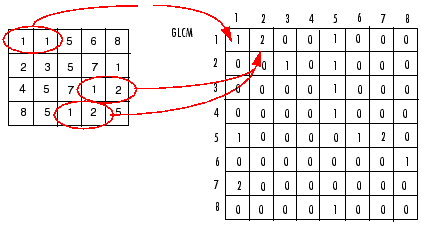
\includegraphics[width=8cm]{GLCM} 
\centering
\caption[Exemplo da elaboração da GLCM]{Exemplo da elaboração da GLCM\protect\footnotemark.}
\label{fig:GLCM}
\centering
\end{figure}
\footnotetext{Extraída de \url{https://www.mathworks.com/help/images/ref/graycomatrix.html}.}
Uma vez criada a matriz de co-ocorrência, diversas medidas podem ser extraídas. Para esse trabalho são extraídas as quatro características definidas abaixo. Nas equações apresentadas $P_{(a,b)}$ representa o valor do elemento na posição $(a,b)$ da GLCM, $\mu_a$ e $\mu_b$ representam a média dos valores de $a$ e $b$ respectivamente e $\sigma_a$ e $\sigma_b$ os desvios padrão destes valores.

\begin{itemize}

\item \textbf{Contraste}: mede o contraste entre um \textit{pixel} e seu vizinho na imagem. Deve ser 0 para uma imagem completamente homogênea. Definido por:
	\begin{equation}
		C = \sum_{a,b} (a-b)^{2}P_{(a,b)}
	\label{eq:Contraste}
	\end{equation}
	
\item \textbf{Correlação}: mede a taxa de correlação de um \textit{pixel} e seu vizinho na imagem inteira. Definida por:
	\begin{equation}
		Co = \sum_{a,b} \frac{(a - \mu_a)(b - \mu_b)P_{(a,b)}}{\sigma_a\sigma_b}
	\label{eq:Correlacao}
	\end{equation}
	
\item \textbf{Energia}: soma do quadrado dos elementos da imagem. Definida por:
	\begin{equation}
		E = \sum_{a,b} P_{(a,b)}^{2}
		\label{eq:Energia}
	\end{equation}
	
\item \textbf{Homogeneidade}: mede a proximidade da distribuição dos elementos à diagonal da matriz. Definida por:
	\begin{equation}
		H = \sum_{a,b} \frac{P_{(a,b)}}{1+|a-b|}
		\label{eq:Homo}
	\end{equation}

\end{itemize}


\subsection{Vídeos}\label{sec:video}


Quando observamos uma cena no mundo real, a cena raramente é estática. Com o passar do tempo, os objetos presentes na cena se movem continuamente pelo espaço, criando infinitas imagens diferentes em nossas retinas. Podemos simular essa sensação de movimento na nossa visão através da exibição rápida de imagens que contém valores discretos. Esse é o conceito de um vídeo digital. Um vídeo digital é formado através da amostragem de imagens	em três eixos: horizontal, vertical e temporal~\cite{LivroVideoDigital,bovik2010handbook}. A cada intervalo fixo de tempo, uma imagem representada por uma matriz bidimensional de valores de intensidade luminosa e cor é amostrada. Cada uma dessas imagens, ou quadros, representa o estado da cena naquele momento no tempo.

\subsubsection{Fluxo Óptico}\label{sec:fluxooptico}

O movimento é um dos elementos principais para a extração de informações de um vídeo. O fluxo óptico~\cite{mota2011tensor}, ou \textit{optical flow}, é uma das técnicas para a estimativa de movimento em vídeos digitais. A técnica consiste em medir a projeção 2D no plano da imagem de um movimento real 3D. Essa projeção 2D mede a velocidade de cada \textit{pixel} da imagem. Esses vetores de velocidade da imagem podem ser utilizados para a realização de diversas tarefas. Por exemplo, é possível extrair a magnitude dos vetores e criar uma nova imagem, aonde os valores de intensidade representam o movimento realizado pelo \textit{pixel}. Nesse trabalho, essa técnica é utilizada para a segmentação de objetos em movimento contra um fundo estático, detalhada no Capítulo \ref{cap:solucao}. A Figura \ref{fig:fluxo} mostra os vetores de movimento calculados e uma imagem em níveis de cinza que representa as magnitudes das velocidades de cada pixel.

\begin{figure}
 \centering
\begin{subfigure}{.5\textwidth}
  \centering
  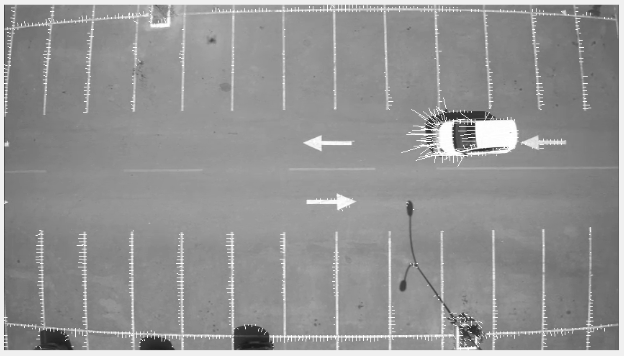
\includegraphics[width=.8\linewidth]{velocidadevetores}
	\caption{}
	\label{fig:fluxo:sub:vetores}
	\centering
\end{subfigure}\
\begin{subfigure}{.5\textwidth}
  \centering
  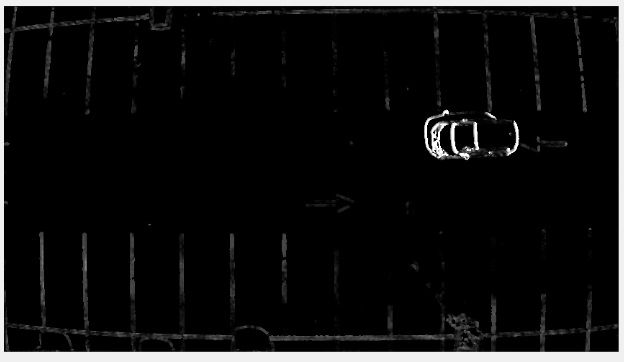
\includegraphics[width=.8\linewidth]{velocidademagnitude}
	\caption{}
	\label{fig:fluxo:sub:magnitude}
	\centering
\end{subfigure}
\caption{(a) Representação dos vetores de velocidade estimada pelo fluxo óptico; (b) Imagem em níveis de cinza onde a intensidade do \textit{pixel} representa a magnitude do seu vetor de velocidade.}
\label{fig:fluxo}
\centering
\end{figure}

Para calcular o fluxo óptico, começamos assumindo que no intervalo entre dois quadros a intensidade de cada \textit{pixel} não muda de forma significativa. Chamamos então a intensidade de cada \textit{pixel} na posição $(i,j)$ em um determinado momento $t$ de $I(i,j,t)$ e portanto, podemos dizer que: 

\begin{equation}
	I(i,j,t) = I(i+di, j+dj, t+dt)
\label{eq:fluxo1}
\end{equation} 

\noindent onde $di$ e $dj$ são o deslocamento que o \textit{pixel} no intervalo $dt$ entre dois quadros.

Queremos então encontrar a velocidade $v =(\frac{di}{dt},\frac{dj}{dt})$ do \textit{pixel}. Usando a expansão por série de Taylor e manipulações matemáticas na Equação \ref{eq:fluxo1}, obtemos a Equação \ref{eq:fluxo2}~\cite{faria1992fluxo}.

\begin{equation}
	\nabla Iv + I_t = 0
\label{eq:fluxo2}
\end{equation}

\noindent onde $\nabla I$ é o gradiente da função intensidade. Essa equação descreve o chamado problema de Restrição do Fluxo Óptico~\cite{mota2011tensor}. Porém, há um problema. A partir da equação só é possível obter um dos componentes da velocidade. A solução completa da velocidade depende de um cálculo na vizinhança de cada ponto. Diversos métodos foram criados para resolver a equação da Restrição do Fluxo Óptico, de naturezas distintas~\cite{mota2011tensor}. Para esse trabalho foi escolhido o método desenvolvido por Lucas e Kanade, detalhado em ~\cite{bruhn2005lucas,faria1992fluxo,mota2011tensor}.

O método de Lucas-Kanade resolve a equação \ref{eq:fluxo2} a partir da suposição que o vetor do fluxo óptico se mantém constante entre os elementos de uma pequena janela imagem. Desta forma é possível elaborar um sistema determinado, que é resolvido por uma aproximação pela técnica dos mínimos quadrados. Apesar de criar uma malha de pontos do campo de velocidade menos densa que outros métodos, o método de Lucas-Kanade é mais resistente a ruídos. Por esse motivo este método foi escolhido para a elaboração do presente trabalho.



%O Capítulo \ref{cap:redes} continua a apresentação de conceitos importantes para o entendimento do trabalho, mas tem foco exclusivo em redes neurais artificiais. 

\subsection{Redes Neurais Artificiais} \label{cap:redes}

Comparado com os computadores mais avançados que existem hoje, o cérebro humano ainda se mostra muito mais poderoso e eficaz do que as máquinas~\cite{Haykin}. O cérebro é capaz de processar informação a uma velocidade muito maior do qualquer computador convencional e realiza com facilidade tarefas como o reconhecimento de padrões e classificação de objetos, enquanto algoritmos tradicionais falham. 

Redes neurais artificiais foram criadas com inspiração no funcionamento e na estrutura do cérebro, como uma alternativa poderosa para resolver problemas que as arquiteturas tradicionais não eram capazes de resolver eficientemente. Essas redes emulam a estrutura cerebral natural, se utilizando de elementos distintos de processamento (neurônios) que se comunicam para realizar a tarefa desejada. 

Simon Haykin define uma rede neural como "...um processador distribuído massivamente paralelo composto por unidades simples de processamento, que possui uma propensidade natural a armazenar conhecimento experimental e torná-lo disponível para uso."

As redes neurais artificiais são utilizadas para resolver problemas como ajuste de funções, classificação de objetos e reconhecimento de padrões~\cite{kohonen1990self}. Esta seção possui explicações e clarificações de conceitos importantes para o entendimento das redes artificiais, começando pelo seu elemento mais básico, o neurônio.

\subsubsection{Neurônios}

O neurônio é a estrutura básica do sistema nervoso~\cite{chiras2013human}. É uma célula composta principalmente de três partes distintas: o corpo celular, os dendritos e o axônio. O corpo celular é a estrutra central do célula aonde está contido o núcleo do neurônio e são executados as suas funções vitais. Os dendritos são prolongamentos do corpo celular responsáveis por receber sinais e o axônio é uma extensão maior do corpo celular, responsável por enviar sinais a outros neurônios. Dois neurônios interagem em apenas  pontos de contato chamados sinapses. Nessas sinapses o axônio de um neurônio envia sinais para os dendritos de um segundo neurônio. A Figura \ref{fig:neuronio} ilustra a estrutura básica dos neurônios.

\begin{figure}
\centering
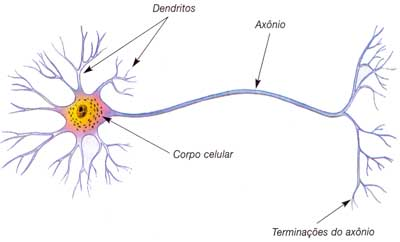
\includegraphics[width=.6\textwidth]{neuronio}
\caption[A estrutura básica de um neurônio humano.]{A estrutura básica de um neurônio humano.\protect\footnotemark}
\label{fig:neuronio}
\centering
\end{figure}

O neurônio artificial também possui três estruturas básicas semelhantes àquelas do neurônio natural. Seus três elementos básicos são: as entradas (análogas aos dendritos), a sáida (análoga ao axônio) e um núcleo de processamento. 
\footnotetext{Extraída de \url{http://www.sobiologia.com.br/conteudos/FisiologiaAnimal/nervoso2.php}.}
O neurônio pode ter uma ou mais conexões de entrada caracterizadas por um peso $w_i$ e que recebe um valor $e_i$. No núcleo do neurônio artificial há um somador que calcula o valor $u$ agregado das entradas, ponderadas pelo peso correspondente. O resultado dessa soma ponderada é então deslocado de um valor escalar e em seguida submetido a uma função chamada de função de ativação, que determina a saída final do neurônio. Em suma podemos descrever a saída de um neurônio $n$ que possui $k$ entradas através das seguintes equações:

\begin{equation}
 u_n = \sum_{j=1}^k e_jw_j
\end{equation}

\begin{equation}
s(n) = f(u_n + d)
\end{equation}

Onde $u_n$ é o valor agregado das entradas, $e_j$ é a j-ésima entrada e $w_j$ o peso da conexão associada, $s(n)$ é a saída do neurônio, $f$ é a função de ativação e $d$ o deslocamento, ou $bias$ do neurônio $n$. A Figura \ref{fig:neuroartificial} ilustra a estrutura básica de um neurônio artificial.

\begin{figure}
\centering
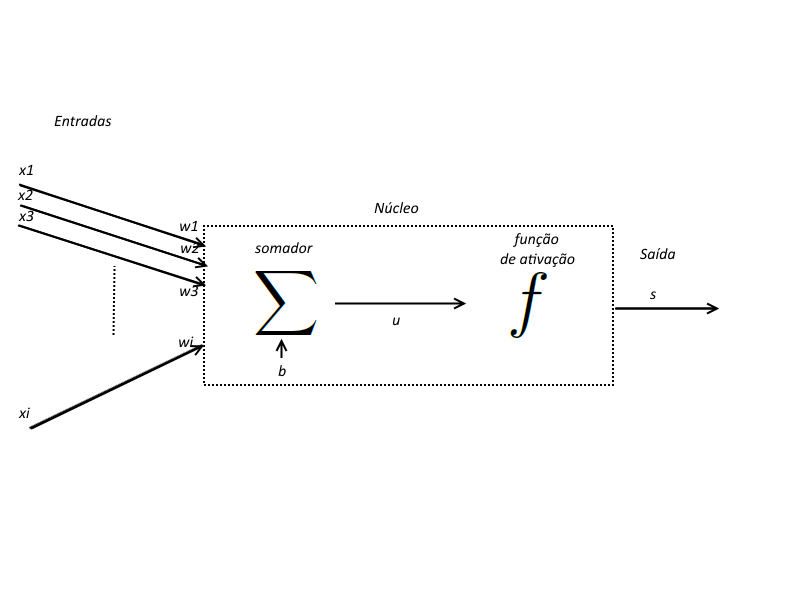
\includegraphics[width=.8\textwidth]{NeuronioArtificial}
\caption{A estrutura básica de um neurônio artificial.}
\label{fig:neuroartificial}
\centering
\end{figure}

Claramente, a função de ativação do neurônio é o grande fator que define o seu comportamento e consequentemente sua funcionalidade. Existem dois tipos básicos de funções de ativação~\cite{Haykin}: a função degrau e a função sigmóide.

O neurônio mais simples possível tem sua saída regida por uma função degrau e saída binária. Isto é, se o valor agregado $u$ de suas entradas for maior que um determinado limiar, a sua saída será 1 e a saída será 0 caso contrário. Apesar de ser capaz de resolver alguns problemas, esse tipo de neurônio tem algumas desvantagens. Por vezes, alterações sutis podem representar a diferença entre os dois valores possíveis da sáida. Além disso, um alcance limitado de valores na saída prejudica o treinamento.

A escolha mais comum de de função de ativação para a construção de redes neurais é a família de funções sigmóides. Essas funções, que tem um gráfico com formato de \textit{S}, assumem valores contínuos entre 0 e 1, o que faz com que alterações sutis na entrada representem alterações mais sutis na saída, aumentando a qualidade da informação gerada pelo neurônio. A mais comum das funções sigmóides utilizadas é a função logística, definida pela Equação \ref{eq:logistica}~\cite{Kosabov}, onde $c$ é uma constante que mede a declividade da curva.

\begin{equation}
	sig(u) = \frac{1}{1 + \exp{-uc}}
\label{eq:logistica}
\end{equation}

Um dos motivos que tornou a função logística uma escolha popular para os neurônios artificiais foi a sua derivação simples, uma vez que algoritmos de treinamento muitas vezes usam a derivada da função de ativação.

É interessante reparar que quando $c$ se aproxima do infinito, a função logística se comporta da mesma forma que a função degrau.

\begin{figure}
 \centering
\begin{subfigure}{.9\textwidth}
  \centering
  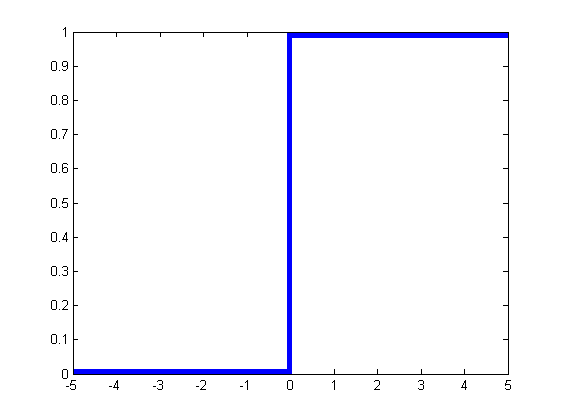
\includegraphics[width=.8\linewidth]{degrau}
	\caption{}
	\label{fig:ativacao:sub:degrau}
	\centering
\end{subfigure}\
\begin{subfigure}{.9\textwidth}
  \centering
  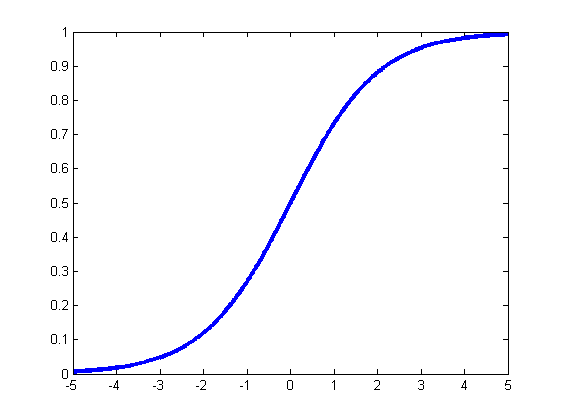
\includegraphics[width=.8\linewidth]{logistica}
	\caption{}
	\label{fig:ativacao:sub:logistica}
	\centering
\end{subfigure}
\caption{(a) Gráfico da função degrau com limiar 0; (b) Gráfico da função logística com a = 1}
\label{fig:ativacao}
\centering
\end{figure}

Outra função de interesse no estudo das redes neurais artificiais, é a função \textit{softmax} ou exponencial normalizada ~\cite{bishop2006pattern}. Essa função é utilizada na teoria estatística para a determinação da distribuição da probabilidade. Isto é, a função \textit{softmax} é uma função que define a probabilidade que uma varíavel discreta assuma um determinado valor~\cite{altmanbs}. Em termos simples, o seu papel é transformar um vetor de $k$ elementos em um segundo vetor de mesmo tamanho, de valores no intervalo $[0,1]$ e que têm soma total igual a $1$.

Essa função é muito utilizada como função de ativação nas camadas de saídas de redes treinadas para reconhecimento de padrões, por sua capacidade de determinar a probabilidade da entrada pertencer a uma determinada classe. A função \textit{softmax} pode ser definida pela Equação \ref{eq:softmax}, onde $vet$ é o vetor de tamanho $k$ da entrada e $vet_i$ é o seu \textit{i-ésimo} elemento.

\begin{equation}
soft(x)_i = \frac{\exp{vet_i}}{\sum_{j=1}^k\exp{vet_j}}
\label{eq:softmax}
\end{equation}




\subsubsection{Redes Neurais Feed-Forward}

Apesar de neurônios serem capazes de resolver alguns problemas sozinhos, o verdadeiro poder das redes neurais vem da interconexão entre os neurônios de forma a criar ligações semelhantes às sinapses dos neurônios naturais.

Existem várias arquiteturas para a formação destas redes de neurônios, porém neste trabalho a discussão será limitada àquela utilizada na implementação do programa: as chamadas redes neurais \textit{feed-forward}.

São necessárias ao menos três camadas para a construção da rede neste modelo: a primeira camada, chamada de camada de entrada, uma ou mais camadas intermediárias (ou ocultas) e a camada de saída. O papel das camadas ocultas é intermediar entre as entradas externas e a saída da rede, de forma a possibilitar que a rede extraia dados estatíticos mais significativos da sua entrada.  Uma camada é composta de um número de neurônios que agem de forma paralela. Cada neurônio de uma camada que não é a de saída está conectado a todos os neurônios da camada seguinte, de forma que não há comunicação entre uma camada e camadas anteriores. Isto é, a informação flui na rede apenas no sentido entrada-saída, como ilustrado na Figura \ref{fig:feedfoward}.

\begin{figure}
\centering
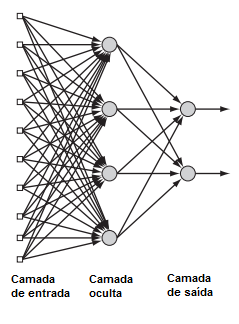
\includegraphics[width=.6\textwidth]{feedforward}
\caption[A arquitetura feed-forward. Cada neurônio se comunica com os neurônios da camada seguinte até que a saída final seja produzida.]{A arquitetura feed-forward. Cada neurônio se comunica com os neurônios da camada seguinte até que a saída final seja produzida.\protect\footnotemark}
\label{fig:feedfoward}
\centering
\end{figure}


\footnotetext{ Adaptada de ~\cite{Haykin}.}
O vetor de entrada da rede é alimentado aos neurônios da primeira camada, cuja saída serve de entrada para a segunda camada e assim por diante, até que a última camada seja alimentada pela saída da camada anterior e produza a saída final da rede. 

\subsubsection{Treinamento}
%Para que uma rede neural artificical possa ser utilizada, ela precisa antes aprender a realizar a tarefa para a qual foi criada.%
 Uma rede neural artificial precisa aprender a realizar a tarefa para qual foi criada antes que possa ser utilizada. Para isso a rede precisa ter duas habilidades importantes: de aprendizado e de generalização. Aprendizado é a capacidade da rede de aproximar o comportamento das entradas fornecidas durante o treinamento, enquanto generalização é a sua capacidade de prever e operar sobre dados além do conjunto com a qual foi treinada~\cite{ZhangNNSurvey}.

É necessário então que a rede passe por um processo de treinamento, onde os valores dos pesos $wi$ e os deslocamentos $b$ de cada neurônio são definidos de forma que o funcionamento da rede seja ótimo para a tarefa que se deseja realizar. Para realizar o treinamento de uma rede, o primeiro passo é definir 3 conjuntos distintos de entradas:

\begin{itemize}
	\item \textbf{Conjunto de treinamento:} A rede é submetida às entradas deste conjunto para que seja feita a calibração dos valores da matriz de pesos $W$ e do vetor de deslocamentos $D$.
	
	\item \textbf{Conjunto de validação:} Após uma etapa de treinamento, a rede computa os dados deste conjunto de entradas para validar os valores da matriz $W$ e do vetor $D$ escolhidos até então.
	
	\item \textbf{Conjunto de testes:} Por fim, após o treinamento, a rede é submetida aos dados deste conjunto, a fim de verificar o seu funcionamento correto.
\end{itemize}

Isto é, a cada ciclo de treinamento, a rede ajusta os seus pesos e deslocamentos de acordo com o conjunto de treinamento, e em seguida processa os dados do conjunto de validação. Se for determinado que a rede teve sucesso no processo de validação, considera-se a rede pronta para passar pelo conjunto de testes, aonde a sua capacidade de generalização é testada. A matriz $W$ de pesos gerada durante este processo é uma forma de representação do "conhecimento" da rede. Assim, o aprendizado não é uma característica de cada neurônio, mas sim um processo que ocorre na rede inteira como resultado do treinamento~\cite{Kosabov}.

Existem duas principais maneiras de se executar o treinamento de uma rede.

\begin{itemize}
	\item \textbf{Treinamento supervisionado:} Neste paradigma os conjunto de treinamento e de validação consistem em um grupo de vetores de entrada $e$ e um gabarito de vetores de saída desejado $gab$. O treinamento acontece até que o vetor de saída da rede para uma determinada entrada $e_i$ seja suficientemente próximo do vetor gabarito $gab_i$ correspondete.
	
	
	\item \textbf{Treinamento não-supervisionado:} Neste paradigma a rede apenas recebe um conjunto $e$ de entradas e aprende características intrínsicas do dados contidos no conjunto.
	
\end{itemize}

Uma vez definido o paradigma de treinamento, é necessário definir uma técnica para a análise do erro e alteração dos valores da matriz de pesos $W$ e do vetor $D$ de deslocamentos. Uma das técnicas mais utilizadas é a chamada de \textit{backpropagation}~\cite{DeepLearning, ZhangNNSurvey}. A técnica consiste de uma análise do erro apresentado na saída da rede, que então é utilizada para se percorrer a rede no sentido contrário dos dados modificando os valores de $W$ e $D$ de forma a diminuir o erro na próxima iteração. Essa técnica é muito utilizada para sistemas de treinamento supervisionado, onde o erro é avaliado através de uma comparação da saída da rede com o gabarito fornecido. Uma vez que os valores de $W$ e $D$ param de mudar, diz-se que a rede atingiu um estado de convergência ~\cite{Kosabov} e o treinamento finaliza.


\subsubsection{Classificação de padrões}




Um problema muito comum que pode ser solucionado com redes neurais artificiais é o da classificação de padrões. Isto é, analisar um padrão ou um conjunto de características de um conjunto de dados e designá-lo a uma de várias classes pré-determinadas. Os nossos sentidos são muitas vezes capazes de fazer isso com extrema facilidade em uma fração de segundo. Por exemplo, se estamos andando pela rua, somos capazes de dizer que um som mais agudo e melódico é o canto de um pássaro, enquanto um som mais grave e contínuo provavelmente pertence ao motor de um carro passando. Essa habilidade é adquirida através de um aprendizado que ocorre durante as nossas vidas, e da mesma forma podemos ensinar uma rede neural artificial a reconhecer e classificar padrões.

Normalmente, uma rede que será utilizada para classificar padrões passa por um treinamento supervisionado, onde é alimentada com um vetor de entradas que contém características que descrevem os padrões junto com um gabarito que determina a classe a qual cada entrada pertence. Espera-se que depois do treinamento, ao ser apresentada a um novo padrão, a rede seja capaz de determinar a qual classe esse padrão pertence. Para que a rede demonstre boa generalização, é importante que a rede não aprenda uma representação exata do conjunto de treinamento, mas que construa um modelo estatístico do processo que gera os dados ~\cite{NNForPR}.

\begin{figure}[!ht]
\centering
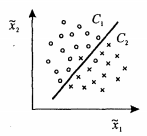
\includegraphics[width=5cm]{features}
\caption[Um gráfico que mostra duas características $\tilde{x}_1$ e $\tilde{x}_2$ de um problema de classificação hipotético.]{Um gráfico que mostra duas características $\tilde{x}_1$ e $\tilde{x}_2$ de um problema de classificação hipotético.\protect\footnotemark  Círculos são padrões da classe $Cl_1$, enquanto os 'x' são padrões da classe $Cl_2$. O limiar de decisão, representado pela linha, consegue separar bem as duas classes quando as características são consideradas como um par. Porém haveria grande sobreposição se os valores fossem considerados separadamente.}
\label{fig:features}
\centering
\end{figure}
\footnotetext{ Extraída de ~\cite{NNForPR}.}
A escolha das características a serem utilizados para descrever os padrões não pode ser aleatória. Deve se escolher um número de características suficiente para descrever todos os padrões que podem ser encontrados. Além disso é importante que as características sejam suficientemente discriminantes. Isto é, deve haver o mínimo possível de superposição entre as características de classes distintas. Essas características podem ser escolhidos a mão, com base em um conhecimento prévio dos dados a serem classificados, ou extraídos automaticamente por um algoritmo desenvolvido para tal. Normalmente as características são processadas em conjunto e não consideradas individualmente. A Figura \ref{fig:features} mostra como isso é benéfico. Se as características hipotéticas $\tilde{x}_1$ e $\tilde{x}_2$ forem consideradas separadamente, há significativa superposição, de forma que é difícil separar com convicção as duas classes $Cl_1$ e $Cl_2$, porém, quando consideradas juntas, é possível traçar uma linha que as separa facilmente, apesar de alguns poucos elementos se confundirem. O papel da rede é determinar a função que traça essa linha através do treinamento, e retornar uma probabilidade de que um conjunto de características que lhe foi fornecido faça parte de uma determinada classe.



Um exemplo: se queremos criar uma rede que diferencia imagens de peixes palhaço de imagens de tubarões, um conjunto adequado de características provavelmente envolveria a cor $c$ predominante do animal, o tamanho do animal $tam$ e o tamanho $bar$ das suas barbatanas. A rede então seria submetida a entradas na forma de um vetor $(c, tam, bar)^T$, valores numéricos que caracterizam uma imagem a ser analisada. Podemos facilmente separar as classe através dessas características. Peixes com cor mais próxima do laranja e barbatanas pequenas são muito provavelmente peixes palhaços, enquanto aqueles que têm a barbatana grande seriam classificados como tubarões.


\section{Trabalhos Correlatos} \label{cap:trabalhos}

Nesse capítulo serão expostas soluções para o problema apresentado no Capítulo \ref{cap:intro}, acompanhadas de uma discussão sobre vantagens e desvantagens, e as razões pela escolha da solução proposta no Capítulo \ref{cap:solucao}.

Podemos separar os métodos de detecção de vagas em duas grandes categorias: métodos intrusivos e não-intrusivos. Métodos intrusivos são caracterizados por exigirem instalações mais complexas, envolvendo a inserção de equipamento no asfalto do estacionamento ou em um estrutura de concreto. Os métodos não intrusivos normalmente se utilizam de equipamentos externos, que não exigem obras para a sua instalação.

Um exemplo comum de método intrusivo é o uso de sensores individuais em cada vaga do estacionamento. Diversos tipos de sensores podem ser utilizados, cada um com vantagens e desvantagens próprias \cite{idris09}. Sensores infravermelhos versáteis e de simples instalação, mas podem ser afetados por condições ambientais. Tubos pneumáticos e sensores de peso sob o asfalto têm alta cofiabilidade, mas exigem grandes obras para a instalação. 

Alguns tipos de sensores podem ser instalados de forma não intrusiva. Esses sensores podem ser afixados no teto ou em uma estrutura próxima a vaga. Sensores ultrassônicos por exemplo, pertencem a essa categoria. Esses sensores transmitem ondas sonoras de baixa frequência e usam a energia refletida para determinar a ocupação das vagas \cite{kianpisheh2012smart}.

Intrusivos ou não, os métodos de detecção que utilizam sensores compartilham duas desvantagens: é necessário a instalação do sensor em cada uma das vagas, aumentando o custo do sistema e diminuindo sua escalabilidade, e eles não são adequados para estacionamentos descobertos, onde é impossível instalar sensores no teto e obras no asfalto rodoviário podem danificá-lo permanentemente \cite{idris09}.

Uma solução que se mostrou adequada para os estacionamentos descobertos foi o uso de \textit{softwares} de visão computacional, que analisam imagens de câmeras de vídeo para determinar a ocupação das vagas do estacionamento. Essa opção tem um custo baixo e exige apenas que sejam instaladas câmeras em pontos estratégicos do estacionamento. Uma vez que as câmeras foram instaladas e as imagens estão sendo capturadas, resta que seja executado um programa que as analise.

Para a escolha da abordagem para este trabalhos foram escolhidos os seguintes critérios principais:

\begin{itemize}
	
	\item O sistema deve poder ser instalado e começar sua execução em um estacionamento em qualquer estado, sem a necessidade de iniciar com todas as vagas descocupadas, possibilitando uma instalação a qualquer momento, sem interrupção das operações do estacionamento.
	\item O sistema deve necessitar de interação humana mínima, se limitando apenas uma rápida calibração no início de sua execução a fim de evitar erro humano.
	\item O sistema deve ser capaz de identificar a posição das vagas do estacionamento após um certo tempo de execução, e não através de entrada manual, para compensar por erros na calibração.
	\item O sistema deve, além de determinar o número de vagas livres no estacionamento, ser capaz de indicar a posição aproximada de tais vagas de forma a facilitar ainda mais a busca por uma vaga desocupada.
	
\end{itemize}

Em \cite{delibaltov2013parking}, Delibaltov \textit{et al} descrevem um método de detecção que estima um volume tridimensional para cada vaga marcada na imagem e depois se utiliza de redes neurais para determinar \textit{pixels} da imagem pertencentes a veículos. Em seguida a sistema computa a probabilidade de que uma certa vaga esteja ocupada baseado em uma função de probabilidade e os \textit{pixels} de veículo na região de interesse de cada vaga. Esse método se mostra preciso e eficaz, mas exige que o estacionamento esteja vazio e que cada vaga seja marcada individualmente no momento de execução, de forma que ele não é capaz de mapear as vagas do estacionamento ou detectar veículos estacionados irregularmente.

Bong \cite{bong2008integrated} propõe um sistema que se utiliza de subtração de imagens e o uso de detecção automática de coordenadas aproximadas das vagas para resolver este problema. Porém esse sistema exige que seja armazenada uma imagem do estacionamento completamente vazio, além de que seja criada uma imagem que marca cada vaga para o processo de inicialização do sistema.

Um sistema que se utiliza de uma técnica de classificação de histogramas de crominância em áreas de interesse e um algoritmo de que encontra pontos com \textit{features} relevantes foi proposto em \cite{true2007vacant}. Esse sistema tem a vantagem de ser relativamente invariante quanto a iluminação da imagem, por utilizar os canais de crominância para a análise. Também é bastante capaz de resolver o problema de oclusão de veículos atrás de outros na imagem de câmeras com uma angulação maior.

A solução proposta neste trabalho procura compensar alguns dos problemas presentes nos trabalhos mencionados, enquanto apresenta uma nova abordagem a ser considerada e aprimorada por trabalhos futuros.








